\chapter{Implementation}\label{ch:implementation}

This chapter presents the created platform; it is structured somewhat similarly to the previous one - firstly, the
audio processing, representation, and transfer are discussed, then both the Backend and Frontend are introduced,
lastly, the deployment process is shown.
In addition, UML diagrams are provided as an overview of the system.

A high-level overview can be seen in the following~\ref{fig:system_overview},
~\ref{fig:Backend},~\ref{fig:Frontend} diagrams.

\begin{figure}[htbp]
    \centering
    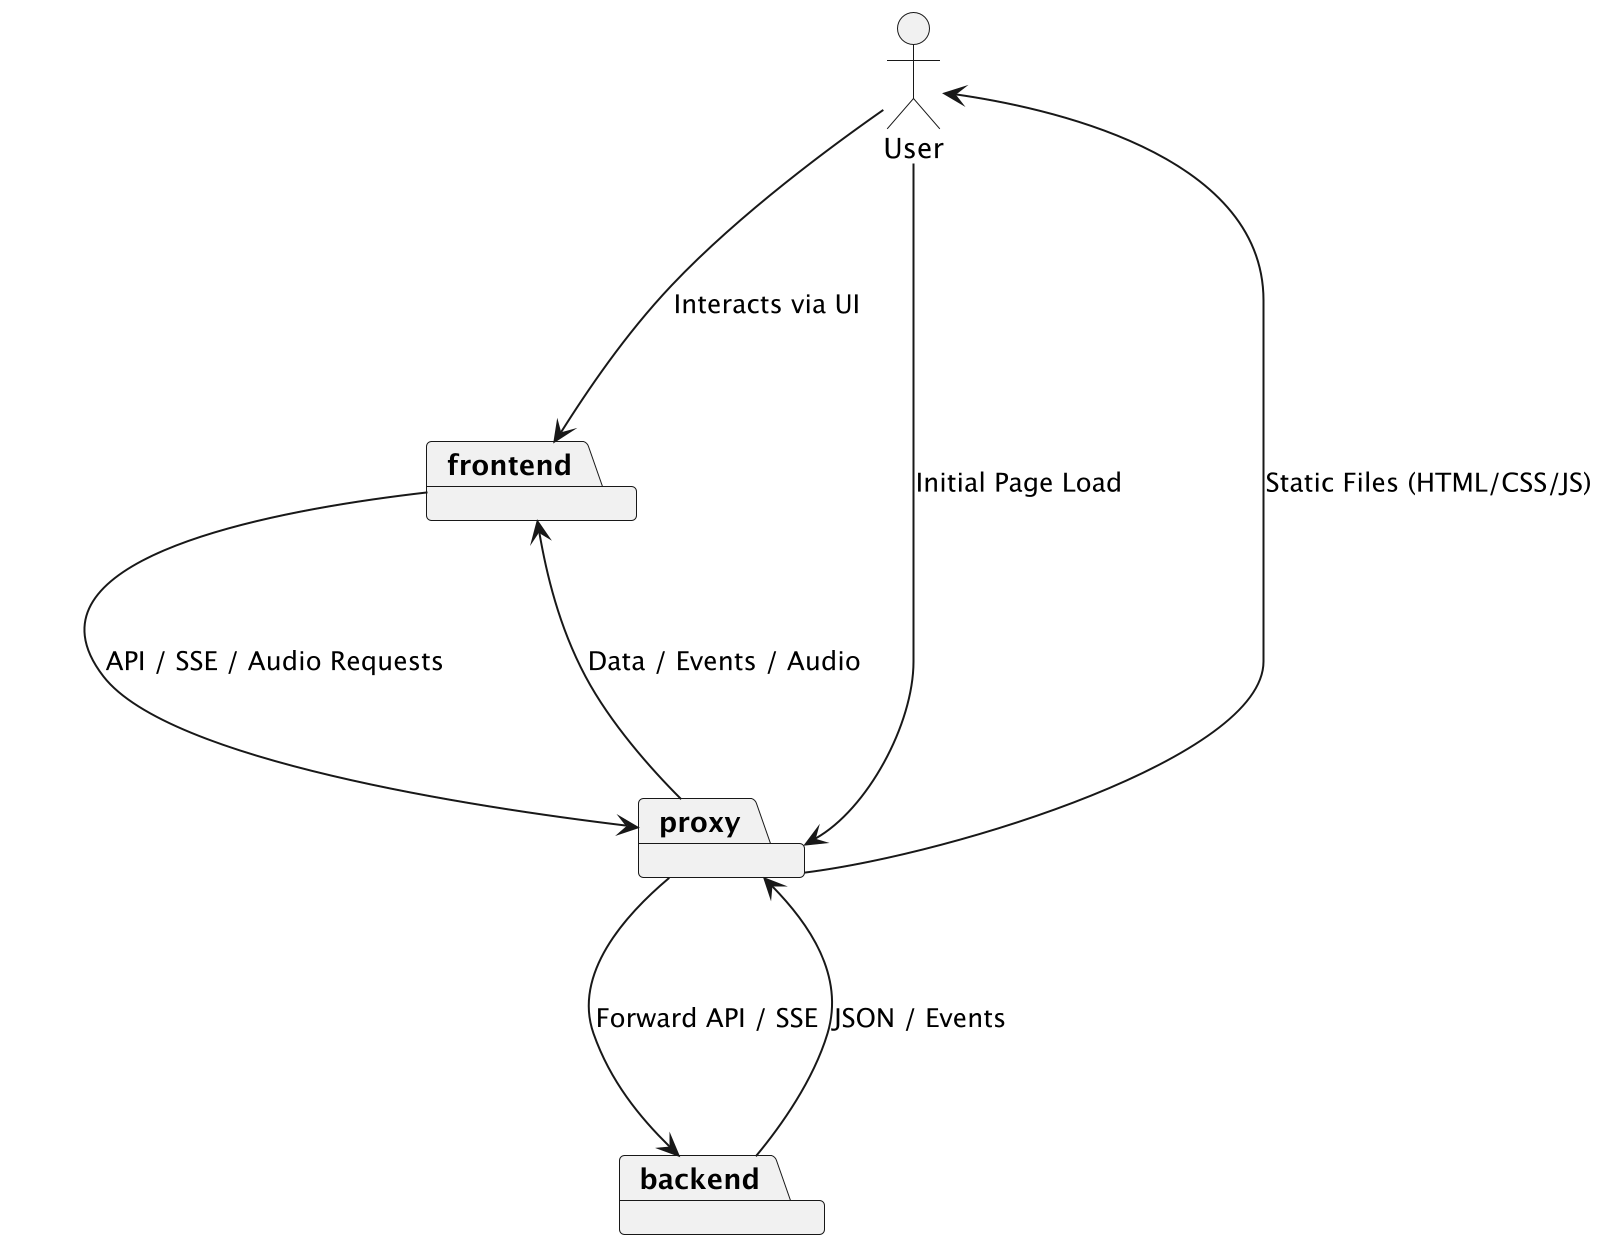
\includegraphics[width=1\textwidth, keepaspectratio]{diagrams/system.png}
    \caption{System Overview}
    \label{fig:system_overview}
\end{figure}

\begin{figure}[htbp]
    \centering
    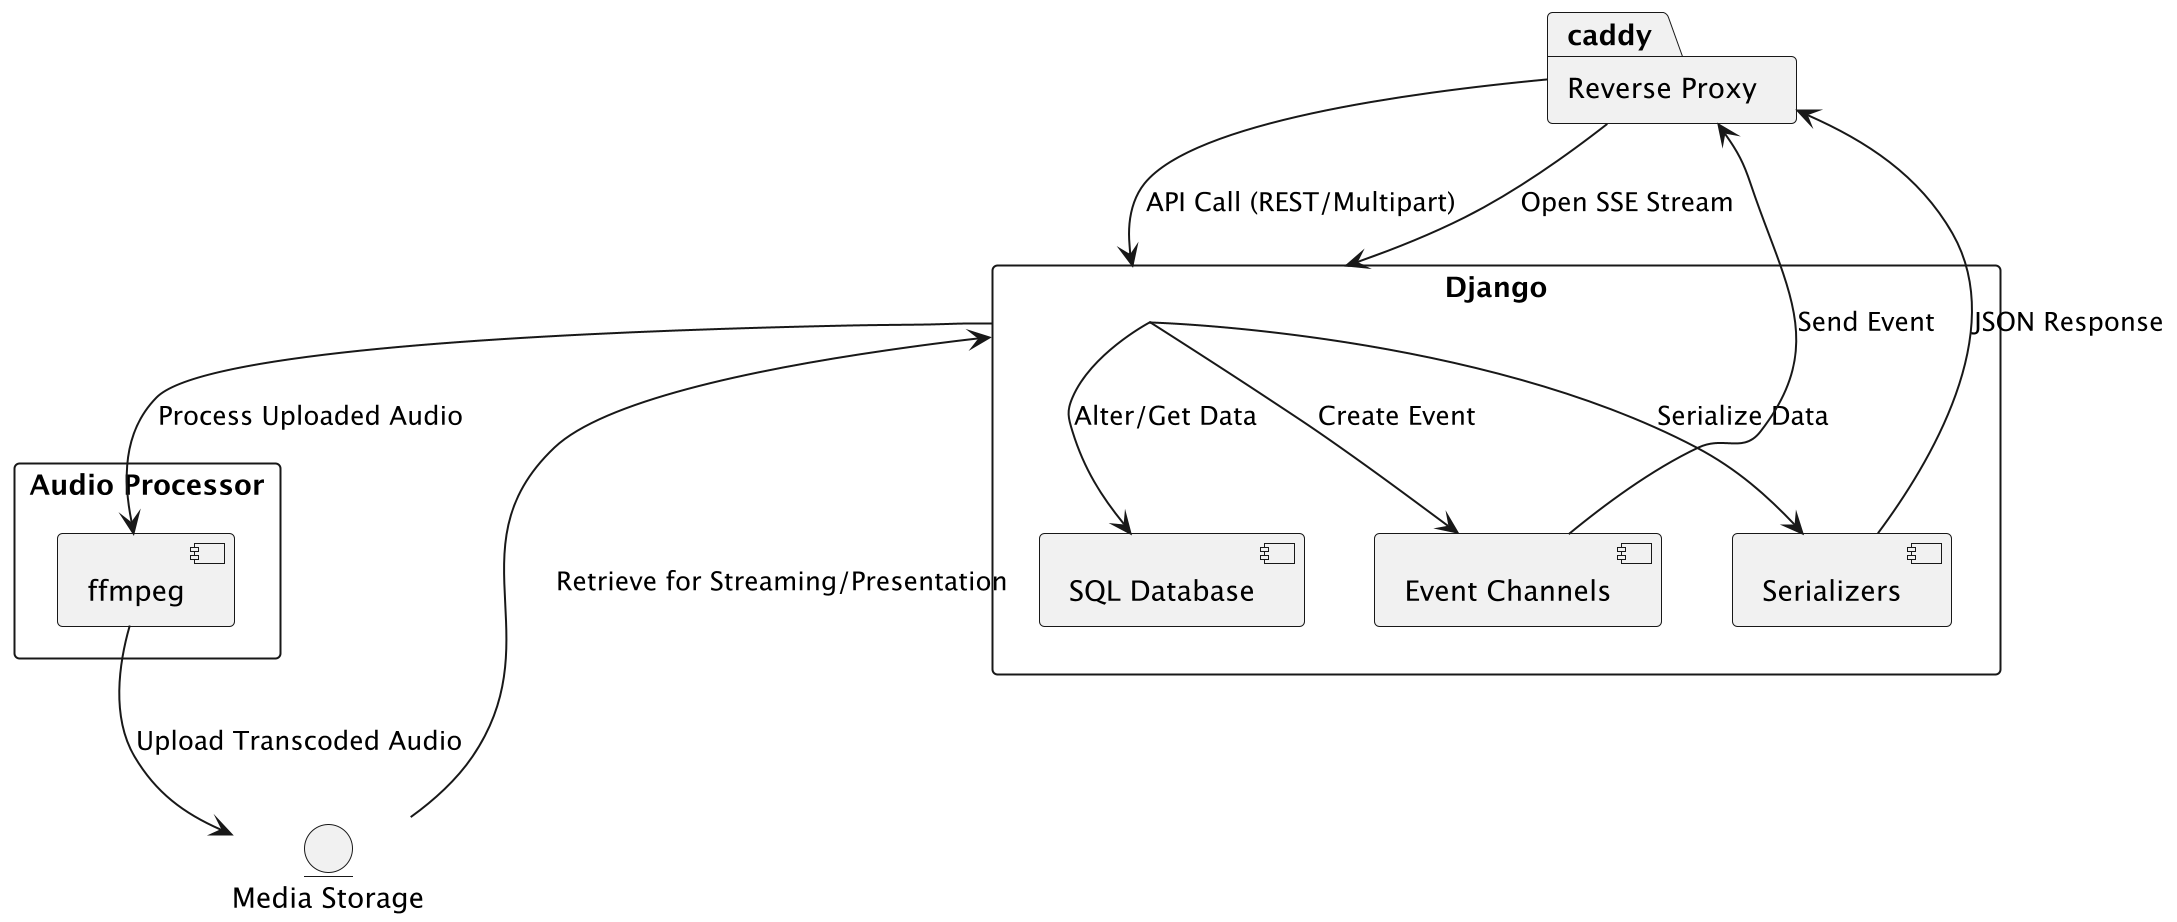
\includegraphics[width=1\textwidth, keepaspectratio]{diagrams/backend.png}
    \caption{Backend}
    \label{fig:Backend}
\end{figure}

\begin{figure}[htbp]
    \centering
    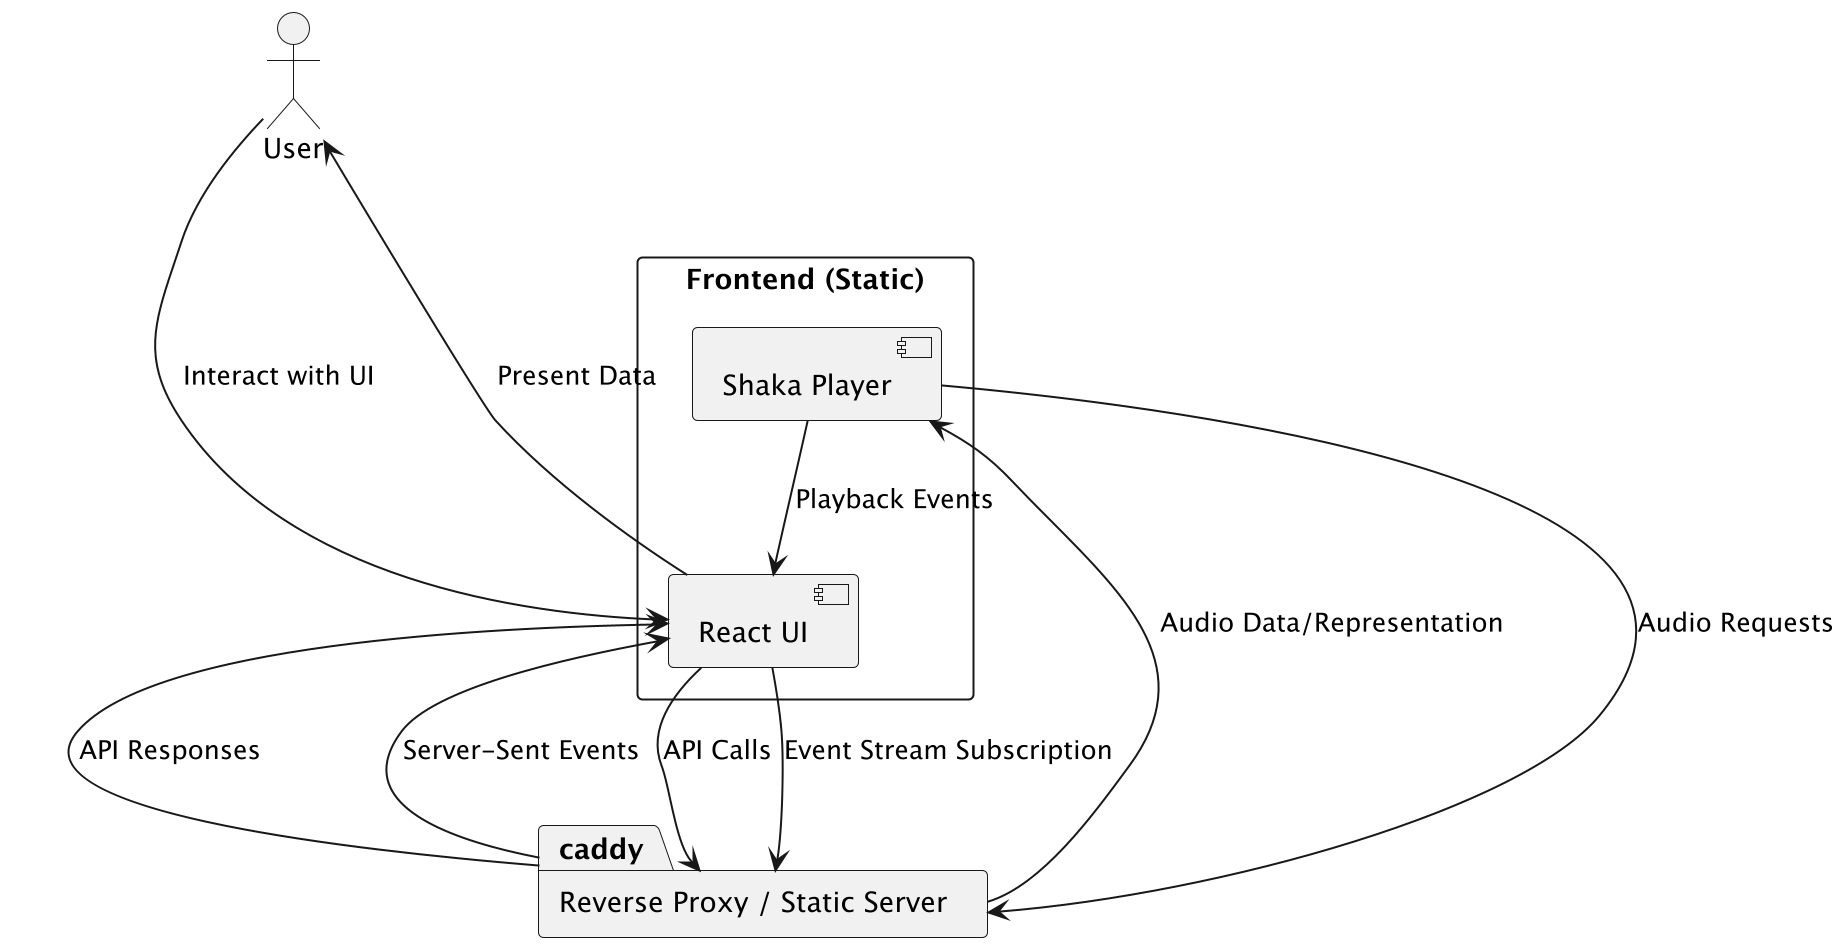
\includegraphics[width=1\textwidth, keepaspectratio]{diagrams/frontend.png}
    \caption{Frontend}
    \label{fig:Frontend}
\end{figure}


\section{Audio Processing, Representation and Transfer}
The most important part that had to be implemented was the audio-related functionality,
hence, the application development began with it.

Below, the core aspects of handling audio are described —-
beginning with the selection of streaming protocols,
followed by how audio is represented and converted into streamable formats,
and finally, the tools and approaches used for processing the audio into the desired
output suitable for web delivery.

\subsection{Streaming Protocols}
Two protocols were chosen for audio streaming - DASH\cite{dash} and HLS\cite{hls}.
Broadly speaking, they work by breaking the initial audio file into smaller chunks and presenting them via a manifest,
which is a listing with all available chunks separated by their timecodes. Then, it is possible to use that manifest
to request individual chunks instead of fetching the whole file. Moreover, it is possible to use
different coders and bitrates for the initial file, which would all be arranged together in the resulting manifest, giving
the possibility to choose which chunk will be served next - e.g., in the case of web audio players, the next chunk can
be chosen based on multiple parameters, for example, network conditions.

At first, only DASH was considered, as it is codec and container agnostic,
is more efficient for lower bitrates, can stream lossless audio(HLS can only on Apple devices),
has multiple DRM implementations to choose from and many further advantages.
However, Safari does not support it well, and on iOS below 17.1, it does not work due to
Media Source Extensions~\cite{mse,msecaniuse} not being present.
Since Safari is the second most used browser~\cite{browserusage}, HLS is also used.

After choosing the streaming protocols, it is necessary to find a way of converting audio to formats that
they support. Audio representation is discussed first, followed by tools for the actual audio processing.

\subsection{Representation}
Usually, when audio is recorded, it is initially saved in lossless formats, which are big due to
the absence of any compression. For instance, the resulting WAV file for 3-minute stereo audio
recorded with a bit depth of 24 bits and a sample rate of 41khz is approximately 42 megabytes, which makes
it very impractical for over-the-net streaming.

Codecs are special programs that aim to reduce the size
while compromising audio quality as little as possible. Most often, they take in multiple input parameters, which affect the resulting converted audio. Among them is bitrate; the initial bitrate for the raw recorded audio
can be calculated as `Sample rate x Bit depth x Number of channels`.
However, codecs typically use bitrate as a primary input parameter instead of those individual components.
This is because bitrate directly controls the trade-off between audio quality and file size,
making it easier to manage encoding and playback requirements.
It also abstracts away the internal implementation details, especially in lossy codecs like AAC or Opus,
which use perceptual models and compression techniques that are not strictly tied to sample rate or bit depth.

In this implementation, Opus and AAC were selected due to their broad support across platforms and
good performance in web-based streaming scenarios.

Opus is a relatively newer codec designed for efficient, low-latency audio transmission over the Internet.
It has superior compression quality compared to other major codecs(including AAC)\cite{opusefficiency},
and often offers better space efficiency.
Additionally, it is open and royalty-free, making it a good option for audio encoding.
However, browser support is not universal—most notably, Safari offers limited support for Opus\cite{caniuseopus},
which restricts its use in HLS.

AAC, in contrast, is an older and more widely adopted codec,
especially in the Apple ecosystem, where it is natively supported across all devices and
browsers. It is also a high-quality codec\cite{opusefficiency}
and remains a standard in many streaming and media distribution systems.
However, one very notable drawback of AAC is licensing – it is not royalty-free, meaning that commercial use,
particularly involving encoding and distribution of AAC audio (as in streaming platforms),
may require obtaining a license and paying fees to the patent holders via organizations like Via Licensing.\cite{vialicensing}


Before selecting the encoding configuration, it is important to distinguish
between two encoding strategies: \textbf{CBR (Constant Bitrate)}\cite{cbr} and \textbf{VBR (Variable Bitrate)}\cite{vbr}.

CBR keeps the bitrate fixed across the entire audio file, resulting in predictable chunk
sizes and smooth playback during streaming. VBR adjusts the bitrate depending on content complexity,
which can provide better quality at a smaller size compared to CBR but leads to inconsistent segment sizes,
making streaming less stable~\cite{cbrvbrcomp}.

For this reason, a \textbf{multi-CBR setup} was selected.
While slightly less efficient in terms of quality-to-size ratio compared to VBR,
CBR provides much greater reliability and predictability in adaptive streaming environments.

The following configuration, based on the official documentation of the respective codec implementations, was selected:
\begin{itemize}[leftmargin=1.5cm]
    \item \textbf{Opus}: 96, 160, and 256 kbps for DASH
    \item \textbf{AAC}: 96, 160, and 320 kbps for HLS
    \item \textbf{AAC-HEv2}: 24 kbps for both HLS and DASH
\end{itemize}
According to performance measurements provided by the codec developers,
these bitrate values offer an optimal balance between audio quality and file size.
Multiple bitrates are included to support adaptive streaming,
allowing web players to select the most appropriate stream based on current conditions dynamically.

\subsection{Processing}
Audio processing is done via \texttt{ffmpeg}\cite{ffmpeg}, which is a tool that supports both the encoding of audio and the
manifest generation for both streaming protocols. It is written in C and supports multithreading, ensuring high audio conversion speed.

FFMPEG provides multiple codec implementations, out of which \texttt{libfdk\_aac} and \texttt{libopus} were used.
Again, the choices were backed by the documentation details~\cite{libfdkaac,libopus}.

In order to integrate it into the Backend architecture, a small wrapper was written, which can be found in the
\path{audio_processing/ffmpeg_wrapper.py} and \path{audio_processing/converters.py} files; a class diagram is also
provided~\ref{fig:ffmpeg}.

\begin{figure}[htbp]
    \centering
    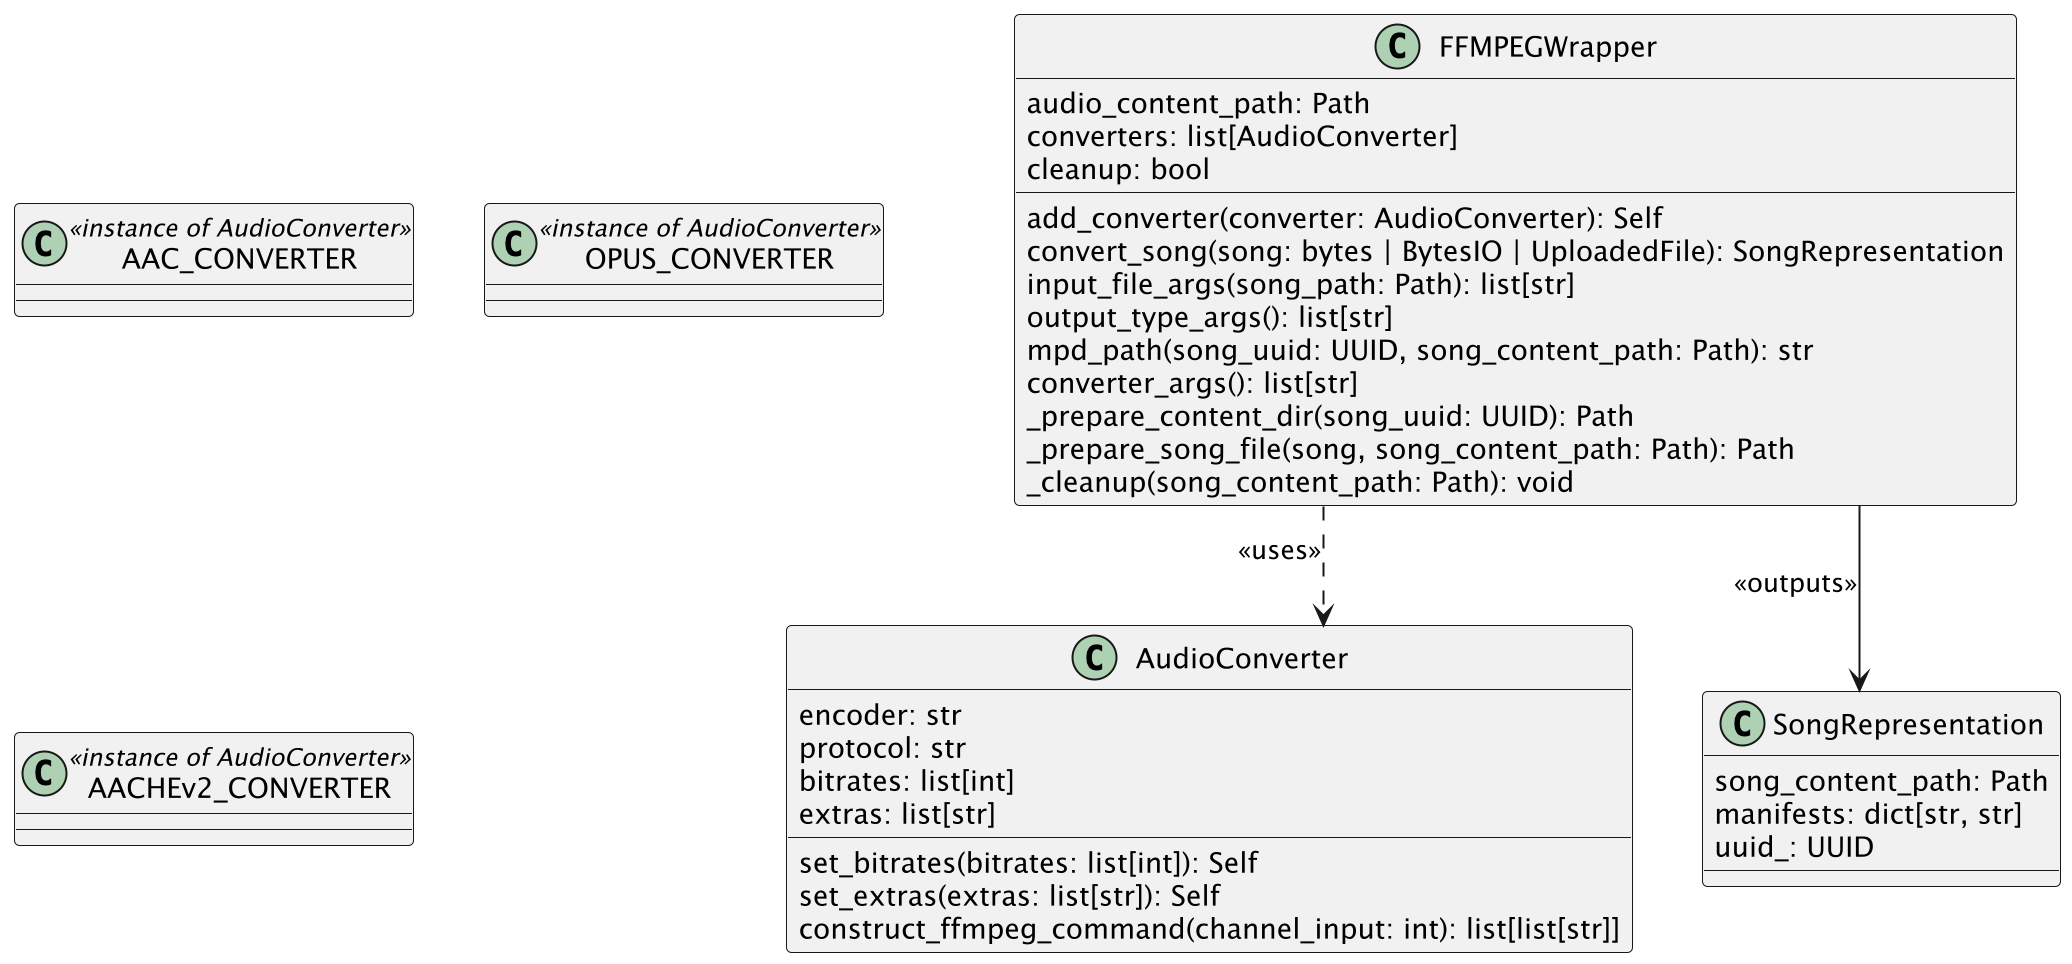
\includegraphics[width=1\textwidth, keepaspectratio]{diagrams/ffmpeg.png}
    \caption{FFMPEG Wrapper}
    \label{fig:ffmpeg}
\end{figure}

There are a couple of packages that have already implemented a wrapper around the library. However,
they are not used because the needed functionality is minimal, and introducing a big
dependency is not necessary. In addition, the more popular and mature package \texttt{ffmpeg-python}\cite{ffmpegpython}
is not maintained anymore, and, e.g., OpenAI has dropped it as their dependency due to that reason\cite{ffmpegopenai}.

The resulting command for \texttt{ffmpeg} constructed by the wrapper(DASH only, for brevity) looks like this:

\begin{minted}{bash}

ffmpeg -i *input file path*
    -map 0:a -c:a:0 libfdk_aac -profile aac_he_v2 -b:a 24k
    -map 0:a -c:a:1 libopus -b:a 96k
    -map 0:a -c:a:2 libopus -b:a 160k
    -map 0:a -c:a:3 libopus -b:a 256k
    -f dash *output file path for manifest*
    -adaptation_sets id=0,streams=a
\end{minted}

\texttt{-map 0:a} tells \texttt{ffmpeg} to select the audio track(s) from the first input.

\texttt{-c:a:*} specifies the codec for each output audio stream.
The index (e.g., \texttt{:0}, \texttt{:1}, etc.) determines the order of the audio representations
in the output DASH manifest.

\texttt{-adaptation\_sets id=0,streams=a} tells ffmpeg to create a single adaptation set that will include all
coded audio streams. That is needed for the ability to switch between them.

As a result, the individual manifests and corresponding chunks are created.
Later, they will be placed under Django's media subdirectory
and prepared to be served to the Frontend audio player.

Having determined how the audio is going to be processed and represented, the data and API model
implementation is discussed in the further section.


\section{Backend}
The description is organized by the individual Django \textit{apps}.
Most of the subsections are comprised of the following parts:

\begin{enumerate}
    \item \textbf{Models} – Objects that define the data schema using Django's ORM.
    \item \textbf{Serializers} – Code that converts Django models or native Python types into
    formats suitable for HTTP transmission (and vice versa).
    \item \textbf{Views} – Handlers for HTTP requests
    that provide the relevant business logic and return appropriate responses.
\end{enumerate}

As a means to simplify the understanding of the underlying architecture, a full class diagram can be
seen first - it encompassed all attributes, methods, and relationships of classes~\ref{fig:beclassdiagram}.

\begin{figure}[htbp]
    \centering
    \begin{adjustbox}{angle=90, width=1.4\textwidth, center}
        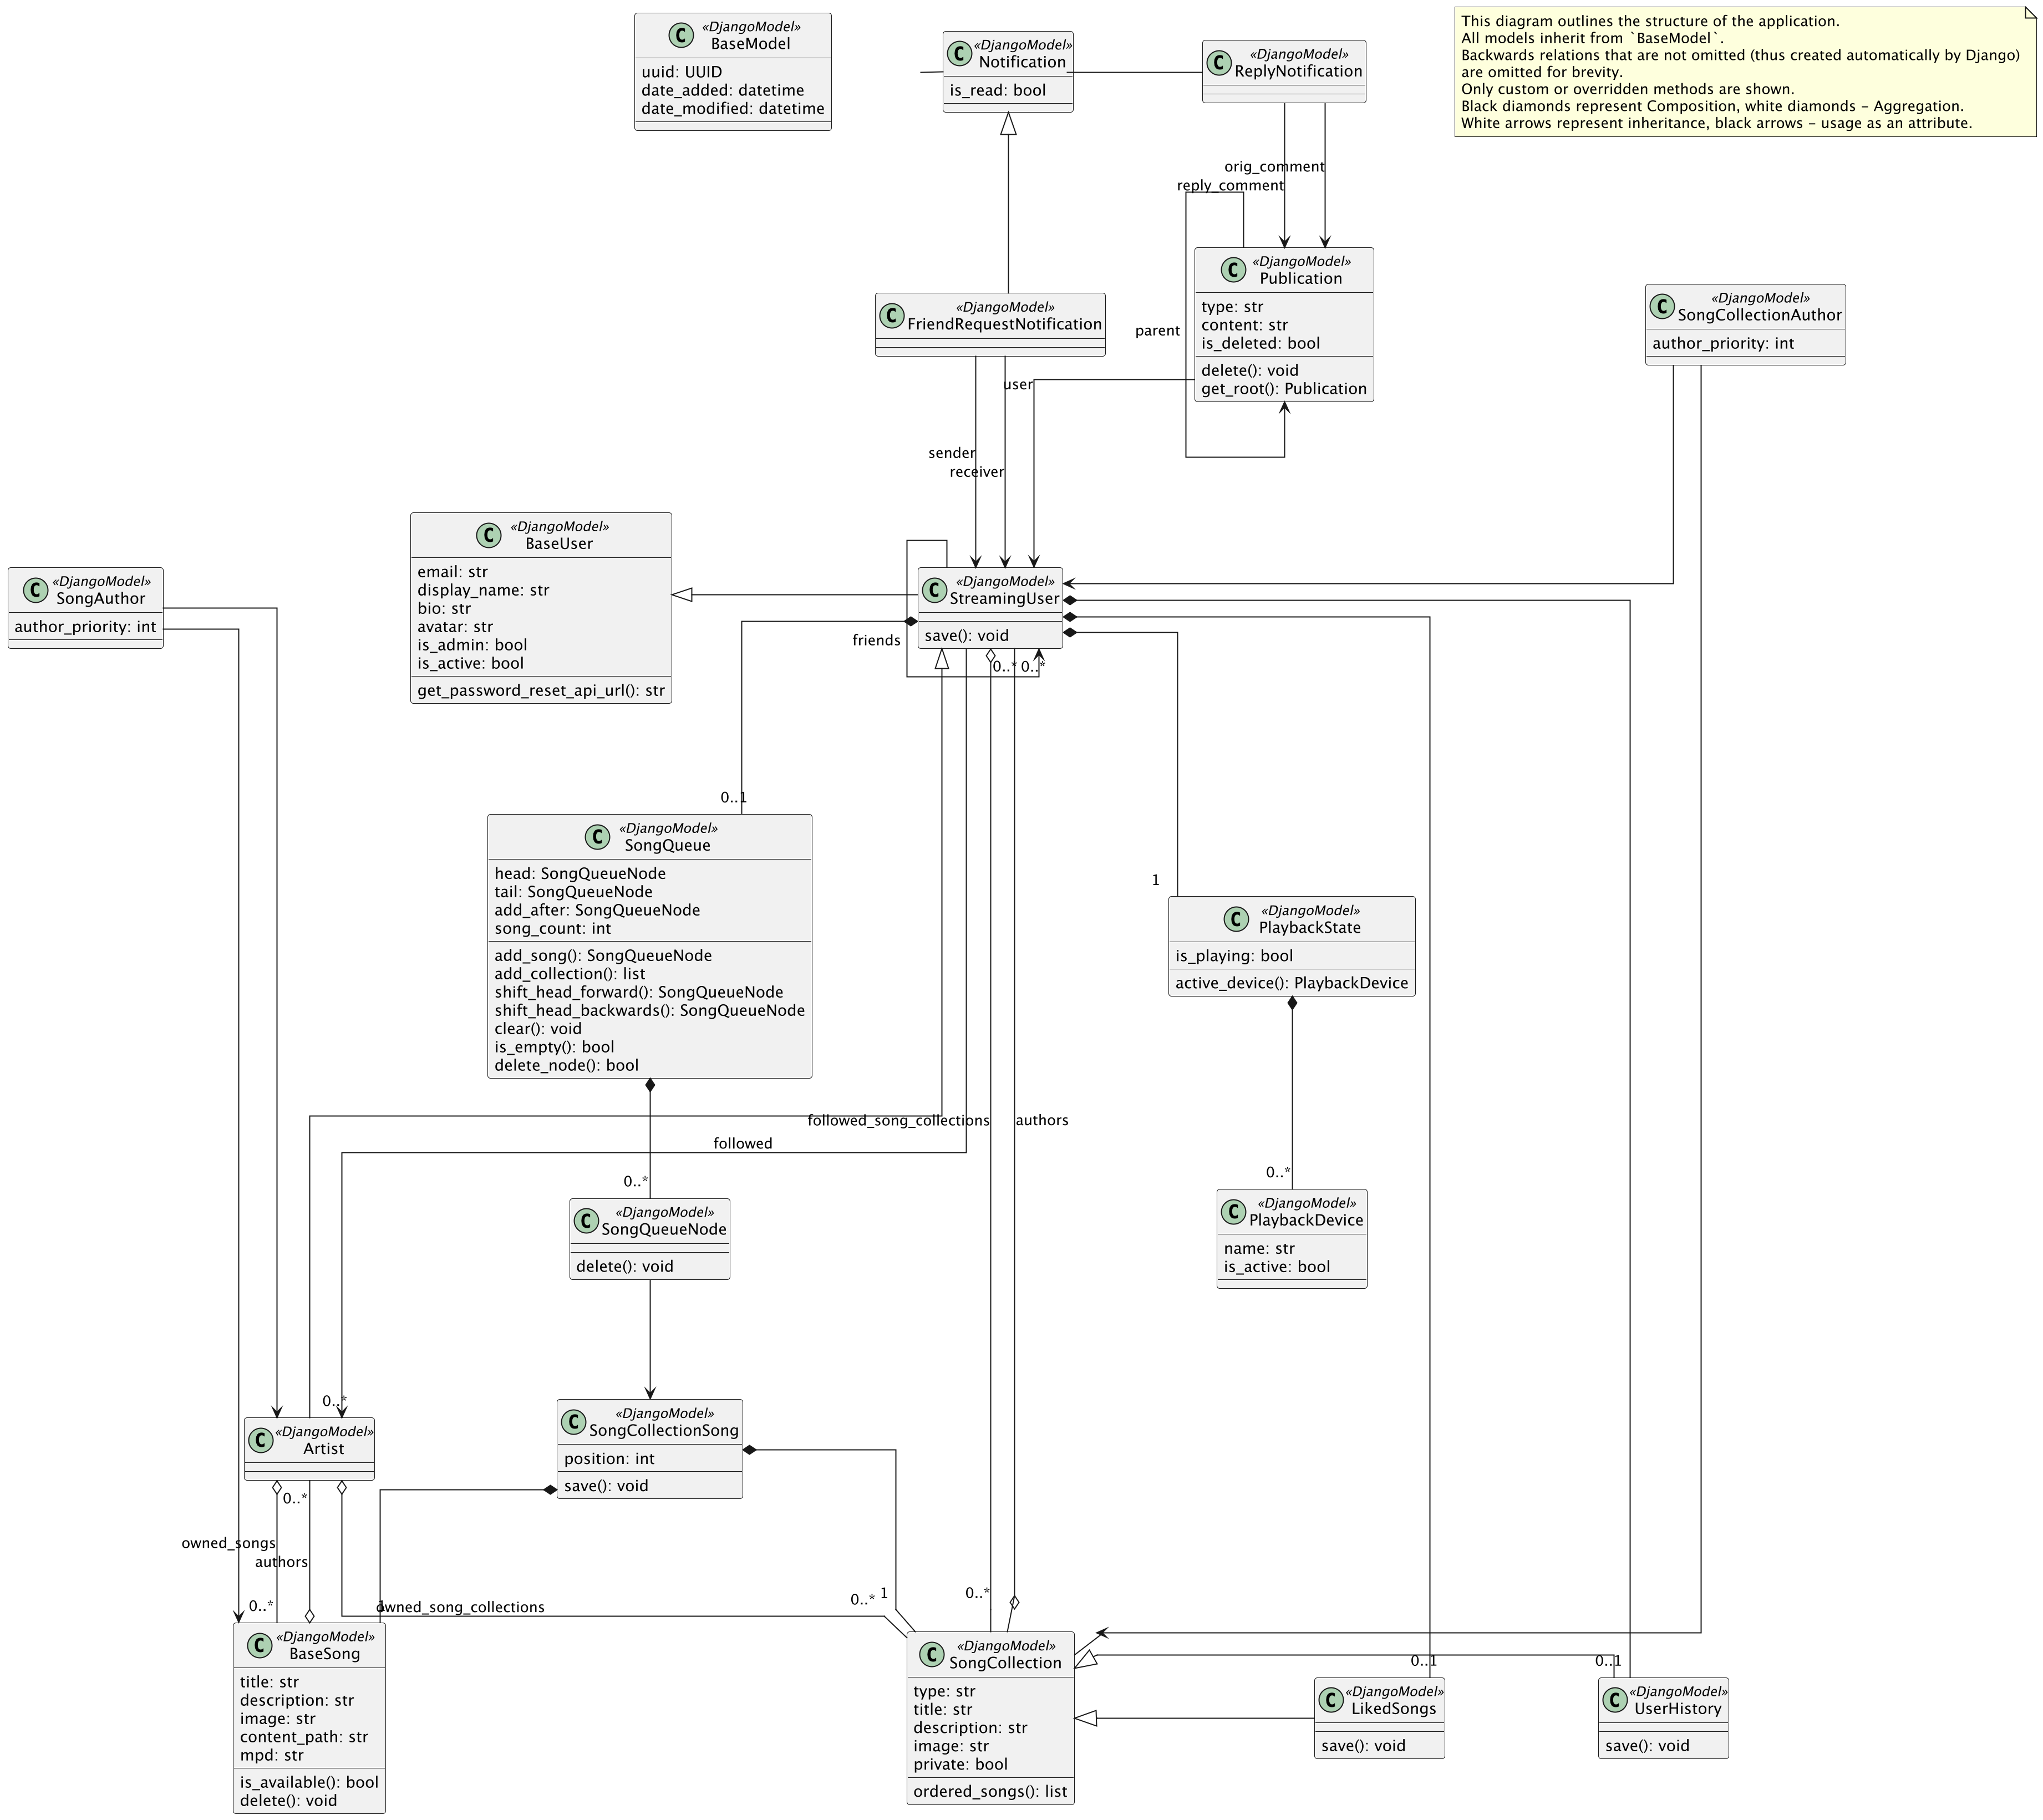
\includegraphics{diagrams/class.png}
    \end{adjustbox}
    \caption{Backend Class Diagram}
    \label{fig:beclassdiagram}
\end{figure}

\subsection{\textit{base}}\label{subsec:base}
This app defines the abstract \texttt{BaseModel} class from which all other models inherit.

It has three attributes - \texttt{uuid, date\_added, date\_modified}. While the latter two are self-explanatory,
\texttt{uuid} has to be explained. Since all the data fetching in Frontend will happen via the REST API,
a unique resource identifier is needed. The drawback of using an \texttt{ID} of the model record,
which is added by default for all models by Django, is the possibility of enumeration attacks~\ref{enumattack}
and unauthorized scraping of the web page. It is much easier to get an existing ID and
simply send requests to API endpoints with an incremented ID value than to guess a random 128-bit string.

A retrieve serializer for the \texttt{BaseModel} is defined as well,
it is also the base class for the serializers of other models.

\subsection{\textit{api}}
Firstly, it is necessary to say that the resulting API follows REST~\cite{restdef} practices; it only deviates from them
when strictly following the rules would degrade the readability and usability of the API.
This can happen, for example, when an endpoint is used to execute an action instead of a data operation.
The other rule that is not followed is the presence of hypermedia links on related resources,
as in the current architecture, it makes more sense to use
individual model identifiers and construct URLs from them instead.

The API itself is versioned, with the current version being \textit{v1}.
In the case of the following apps, all the API-related files are always defined under the \path{api/v1} folder.

As for the endpoint, all views that operate on data in some way require authentication, which can be determined
by the presence of
\\\mintinline{python}{permission_classes = [IsAuthenticated]}\\
attribute on the view. User roles
are also differentiated by checking the existence of the appropriate model, e.g., for Song creation, the User set
on request has to have a corresponding \texttt{Artist} instance.

\subsection{\textit{users}}
User classes and token logic are defined in this app.

There are three main User classes:
\begin{itemize}
    \item \texttt{BaseUser} - declares common fields for all other models, such as \texttt{email, display\_name} and others.
    \item \texttt{StreamingUser} - the main class representing an account with privileges to use the streaming platform.\\
    Additional attributes are declared for it, namely:
    \begin{itemize}
        \item Relations to other users: \texttt{friends}, which are other \texttt{StreamingUsers},\\
        friend requests of whom the user has accepted (or the other way around);\\
        \texttt{followed} - the \texttt{Artist}s to the updates to which the User has subscribed.

        \item User-specific Song Collections: \texttt{history} containing all listened Songs,\\
        \texttt{liked\_songs} containing favourited Songs,\\
        and \texttt{followed\_song\_collections} - the Collections which the user has saved to their profile.

        \item \texttt{song\_queue} - a special structure containing already/to be listened to Songs of the User,\\
        it will be described later in the dedicated app.
    \end{itemize}
    \item \texttt{Artist}: a subclass of \texttt{StreamingUser} with additional capabilities, such as Song uploads.
\end{itemize}

JWTTokens are also customized in this app.
They are based on the implementation from \texttt{djangorestframework-simplejwt}~\cite{simplejwt}.
The token system follows the standard logic of access and refresh tokens:
the access token is short-lived and used to authenticate regular API requests,
while the refresh token is long-lived and can be used to obtain new access tokens without requiring
the user to re-authenticate.

Authentication for each HTTP request involves attaching the access token as an HTTP \textit{Bearer} header.
After parsing the request, the token is retrieved and validated.
After validation, the User identifier is extracted and used to identify the corresponding User record.
User validation logic is changed so it uses User's \texttt{uuid}, hence it is added to the token payload.
This is done for the same reasons outlined in the \nameref{subsec:base}.

Basic serializers for all User models are declared,
allowing for retrieving information about specific Users or their creations and updates.

The following views are added as well:
\begin{itemize}
    \item \texttt{UserRetrieveUpdateView}
    \item \texttt{UserCreateView}
    \item \texttt{UserFriendsView}
    \item \texttt{UserFollowedView}
    \item \texttt{UserFriendsCreateDeleteView}
    \item \texttt{ArtistFollowersView}
    \item \texttt{UserEventViewSet}
\end{itemize}

The purpose of all views, except for the last one, is to send the information
about Users or perform create/update actions on the related data.

UserEventViewSet is a special view used to implement the SSE connection,
the details are provided in the subsection \nameref{sec:sse}.

Views for token generation and renewal have also been declared. Their respective endpoints are:

\begin{itemize}
    \item \texttt{/api/v1/token/} — accepts user credentials (email and password) and returns a
    token pair (access and refresh tokens).
    \item \texttt{/api/v1/token/refresh/} — accepts a refresh token and returns a new access token.
\end{itemize}

\subsection{\textit{sse}}\label{sec:sse}
As was mentioned in \nameref{ch:planning}, \texttt{django-eventstream} package is used for the Server Sent Events
configuration. Internally, it creates special objects called \textit{channels} to which clients can subscribe
via an HTTP request. Then, when a new event for a specific channel is created,
e.g., via the \texttt{django-eventstream.send\_event()} method, all clients subscribed to that channel
will receive an HTTP response with the specified content.

`UserEventViewSet` listens for incoming SSE connection requests from Users and creates a personalized channel using the User's UUID.

Events are used throughout the system primarily to signify to the Frontend that some data is stale.
An example of this is the aforementioned `UserFriendsView`, the post request handler of which is defined like this:

\begin{minipage}{\textwidth}
    \begin{minted}{python}
    class UserFriendsCreateDeleteView(APIView):
    ...
    def post(self, request, *args, **kwargs):
        ...
        user.friends.add(sender)
        send_invalidate_event(
            EventChannels.user_events(user.uuid),
            ["user", "friends", str(user.uuid)]
        )
        ...
    \end{minted}
\end{minipage}
\\
\\
Here, the custom \texttt{invalidate\_event} signifies to the Frontend that the \texttt{friends}
list has changed and should be refetched.

The \textit{invalidate} logic is present for views operating on models used in the Frontend, specifically in view handlers which change data.
That way, the client will always have fresh information.

Event re-delivery is also handled by the package set with this parameter in Django settings:

\begin{flushleft}
    \begin{minted}{python}
    EVENTSTREAM_STORAGE_CLASS = \
        'django_eventstream.storage.DjangoModelStorage'
    \end{minted}
\end{flushleft}

This tells the package to store the events in the database and in case of network failure
or client disconnect they are redelivered.

Since the SSE part has been explained, it is safe to consider the main part of the application
-- the \textit{streaming} package.

\subsection{\textit{streaming}}
This app defines the main models responsible for the audio content and playback handling.

\subsubsection{Songs and Song Collections}
The backbone of the application is the \texttt{BaseSong} and \texttt{SongCollection} models, which are declared
in \path{streaming/songs.py} and \path{streaming/song_collections.py} files.

\begin{itemize}

    \item
    \texttt{BaseSong} contains the metadata about each individual song - \texttt{title},
    \texttt{description} and \texttt{image}.

    Then, there are attributes that contain the information about the underlying song file:
    - \texttt{content\_path} representing the root directory with Song files(chunks, manifests)
    - \texttt{mpd, m3u8} providing manifest paths for DASH and HLS, respectively.

    The last attribute is \texttt{draft}. It is used in the Song creation process, which will be explained in the
    view description.

    \item
    \texttt{SongCollection} represents a container for Songs and can be of two types(set with \texttt{type} attribute)
    -- either a Playlist or an Album.
    A Playlist is a collection formed from existing Songs, which both StreamingUsers and Artists can create. An Album, on the other hand, is a collection that can be created only by an Artist
    containing unique, uploaded Songs.

    Because an individual \texttt{BaseSong} can be in multiple collections, a Many-to-Many relation is defined between
    \texttt{BaseSong} and \texttt{SongCollection} named \texttt{SongCollectionSong}.
    A \texttt{position} attribute is added to enable the arbitrary ordering of the songs.

    Another attribute on the \texttt{SongCollection} is \texttt{comments}.
    As the name suggests, these are pieces of text that each User can add to the collection. The underlying
    model is discussed in the \nameref{subsec:social}.

    The same metadata as in \texttt{BaseSong} can also be set.
    However, there is one extra attribute - \texttt{private}.
    It is used to signify which collections should not appear, e.g., in global search results.

    In addition, there are two subclasses of \texttt{SongCollection} - \texttt{UserHistory} and \texttt{LikedSongs}.
    They are moved to separate classes because, in the future, they will most probably have custom logic added to them.
    In the app's current version, only the ordering that makes the newest added songs appear first is defined.

\end{itemize}

Each \texttt{SongCollection} and \texttt{BaseSong} also has a relation to the Users that created it(and visa versa).
It is defined as an M2M relationship with an intermediary table - \texttt{SongCollectionAuthor} and
\texttt{SongAuthor}. Attribute \texttt{author\_priority} sets the order in which the authors should be returned from
the API and displayed on the Frontend.

As for the views and endpoints - a standard set of CRUD operations is implemented for both models.
Additionally, there are special views for User interactions with models, such as \texttt{SongAddLikedView}, which adds
the provided Song to User's \texttt{LikedSongs} or \texttt{SongCollectionRemoveSong}, which lets the User remove a Song
from a collection, if that User created it.

However, some things have to be said about Song and Collection creation.
The design choice is not to allow users to create isolated Song instances; if the User wants to upload Songs separately from a Collection, a single-song Album would
be created instead. This greatly simplifies the logic when handling User playback interactions later on.
For example, it makes it possible to use the aforementioned \texttt{SongCollectionSong}
instead of \texttt{BaseSong} in most views. As this relation contains the information about both models,
we can, for instance, accurately show not only which Song is playing, but a Collection as well,
without tracking both models.
This has further benefits, which can be seen in the Frontend implementation.
\\
Apart from that, the Collection creation process is multi-stage, and two views are responsible for it:
\texttt{SongCreateView} and \texttt{SongCollectionCreateView}.
Whenever a User wants to create a new Collection, firstly the Songs are processed.
If an error happens during this stage, the response with successful and failed Songs is returned, and \texttt{draft} attribute is set to \textit{True} for the created Songs.
This is done because the User can abort the process of creation, e.g.,
by closing the whole browser application, and there would be no proper way to signal what Songs should be deleted.
A simple crontab job or \texttt{celery} library could be utilized to run periodic tasks which would clean up
Songs in the draft state.
\\
When creating a Song, multiple validation stages are made for the User input, both on the Frontend and the Backend.
For instance, \path{ffmpeg_wrapper.py} checks the audio file size, its mime type via~\cite{pythonmagic} library, and the
underlying format, with available formats specified in \path{ffmpeg_wrapper.ALLOWED_FILE_TYPES} variable.

Having discussed the main building blocks of the audio content part of the application,
\texttt{SongQueue}, which operates on these models, can be presented.

\subsubsection{SongQueue}
\texttt{SongQueue} represents a list of previously listened Songs and the ones that are going to be
listened by the User.

The choice of the underlying structure was made based on the desired operations.
Basic addition and removal from the queue had to be supported, as well as the differentiation
between playing a Song/Collection or adding it to the queue.
For example, when a user clicks play on a Song, it has to become the new "head" of the queue.
In case of clicking "add to queue" this Song would be added after other items
that have been queued previously. This implies that addition/removal can happen in any part
of the list. As a result, a Doubly Linked List pattern has been chosen for this model.

As the queue information had to be persisted in the database, a common implementation with
nodes that point(using foreign keys) to the next and previous node might not have been the most efficient. An interesting approach proposed online was to use a \textit{position} column
instead of foreign key references. That way it would be possible to retrieve the whole queue with an SQL statement
like this:

\begin{minted}{sql}
SELECT *
FROM (join node table, queue table, and StreamingUser table
      to find the queue nodes of a particular User)
WHERE node.position > (join queue and nodes to find the head of the queue)
ORDER BY node.position
\end{minted}

While using a \texttt{position} column simplifies queue traversal and ordering, it introduces potential
issues when it comes to frequent inserts and deletes.

Every time a node is inserted between two existing positions, a new \texttt{position} value must be chosen
such that the ordering remains correct. If positions are represented by integers, repeated insertions
between tightly packed values (e.g., inserting between positions 1 and 2) will eventually require
re-indexing the entire list to free up space. This operation can be expensive in terms of performance.
Similar problems can occur during deletes as well.

These limitations could be mitigated, for example, by using high-precision floating point numbers,
powers of numbers or large increments like 1000 to delay the need for full re-indexing.
However, without the data showing the expected usage of the queue, it is hard to tell whether this approach would
be beneficial.

That is why a more straightforward approach with identifiers of neighboring nodes was chosen, at least for now.

Two models comprise the queue functionality - \texttt{SongQueueNode} and \texttt{SongQueue} itself.

Each node carries information about the \texttt{SongCollectionSong} attached to it, as well as
links to the previous and next node.

\texttt{SongQueue} has foreign keys to the nodes which signify the \texttt{head} and \texttt{tail} of the queue.
Moreover, a special, third attribute is declared - \texttt{add\_after}. This is also
a foreign key to one of the nodes, but this time, it indicates the node after which items
should be added when the "add to queue" action is selected.
I.e. if the user had selected "play" on a Song, it would become the queue head.
Then, if the user selected "add to queue" on five different Songs,
then the head would still point to the playing Song, but \texttt{add\_after} would
contain the key of the fifth Song added using the second action.

Multiple operations are supported, with the main ones being:
\begin{itemize}
    \item Setting the queue head. In the case of Collections, e.g.,
    when the User clicks "play" on a Collection object, the entire Collection is added to the queue.
    \item Shifting the queue head backward and forward.
    \item Removing a node.
    \item Clearing the entire queue.
\end{itemize}


The final aspect that needs to be addressed is managing the playback state.

\subsubsection{Playback State and Playback Devices}
The term "playback" represents the state of the sound, whether it is being played in a given moment.
Each User has an attribute named \texttt{playback\_state} represented by the \texttt{PlaybackState} model.
The playback can be toggled by using the \texttt{PlaybackState.is\_playing} attribute.

Because the User can open multiple instances of an application, the playback handling can not be
unloaded to the Frontend only, as it would not be synchronized across the application instances.

As a result, the application has to differentiate the User's "sessions", which is done
via the \texttt{PlaybackDevice} model.
It represents the individual devices on which the application is currently open.
Each device has \texttt{is\_active} attribute, signifying where the sound should be played and where
to display controls(seek bar, volume).

It would be expected for all instances of the application to show the same playback state(playing/stopped),
and intuitively clicking the play button would have to result in playback being toggled on the active device with
visual confirmation on all other devices. In addition, the active device must be able to be switched, which is done
by the appropriate \texttt{PlaybackDeviceActivateView} handler.

The standard serializers and views allowing state/device manipulation are implemented.
However, \texttt{PlaybackDeviceDeleteView} deviates from the standard rules, as it allows non-authenticated requests
and softens the CSRF restrictions. This is done due to browser limitations, shown in the \nameref{subsec:fedevices}.
The authentication is still made "by hand" inside the handler itself.

This concludes the audio part of the application.

\subsection{\textit{social}}\label{subsec:social}
Before examining the contents of the \textit{social} app, an important Django concept
has to be brought up -- the \texttt{ContentType} framework and \texttt{Generic Relation}~\cite{djangocontenttype}.

The \texttt{ContentType} framework provides a way to refer to any model in the system
using a generic identifier.
\texttt{GenericRelation} uses the \texttt{ContentType} framework by storing the target
model’s type and primary key in two separate fields: a foreign key to the
\texttt{ContentType} model and an object ID.
Together, these allow a single relation to point to any instance of any model,
enabling polymorphic associations without hardcoding specific model references.

This concept is used to implement the \texttt{Publication} model.

For a better understanding, the model code can be found below.
Here, the \texttt{content\_object} field is a \texttt{GenericForeignKey}
that dynamically joins the \texttt{content\_type} and \texttt{object\_id}
fields to establish a reference to any model instance.
This allows each \texttt{Publication} instance to be associated with
an arbitrary object, such as a Song or a Collection, without requiring a
fixed foreign key to a specific model.

\begin{minted}{python}
class Publication(BaseModel):
    class PublicationType(models.TextChoices):
        COMMENT = "comment", "Comment"
        POST = "post", "Post"

    RELATED_MODEL_TYPE_MAP = {
        "user": "users.StreamingUser",
        "collection": "streaming.SongCollection",
        "song": "streaming.SongCollectionSong",
    }

    type = models.CharField(choices=PublicationType.choices)
    content = models.CharField(max_length=255)
    user = models.ForeignKey(
        settings.AUTH_USER_MODEL, null=True,
        on_delete=models.SET_NULL
    )
    parent = models.ForeignKey(
        "self", null=True, blank=True,
        related_name="replies", on_delete=models.SET_NULL
    )
    is_deleted = models.BooleanField(default=False)

    content_type = models.ForeignKey(
        ContentType, null=True,
        blank=True, on_delete=on_content_type_delete
    )
    object_id = models.PositiveIntegerField(null=True, blank=True)
    content_object = GenericForeignKey()
\end{minted}

Another attribute that needs an explanation is \texttt{type}.
Currently, it can have one of two values - \texttt{comment} and \texttt{post}.
The comment type is used for comments under audio content(collections),
while \texttt{posts} represent standalone User publications.

The \texttt{Publication} model also contains a \texttt{parent} attribute, allowing for
building trees of publications(i.e., replies).

Standard CRUD serializers and views for publications are provided,
with the addition of custom handling of the related models.

Views related to the publication creation also have a special handling
of instances that are considered as replies. They create a special
\texttt{ReplyNotification} object, discussed in the next subsection \nameref{subsec:notif}.

\subsection{\textit{notifications}}\label{subsec:notif}
In order to notify users about actions such as replies to their publications
or new friend requests, a notification system was implemented.

The following two notification types are currently supported:
\begin{itemize}
    \item \texttt{ReplyNotification} – created when a user replies to a publication (e.g., comment).
    It stores references to both the original and reply comments. The corresponding manager triggers an SSE
    event to the original author's channel, making Frontend refresh the notifications list.
    \item \texttt{FriendRequestNotification} – created when a friend request is sent.
    It stores references to both the sender and the receiver. Upon creation, same as for \texttt{ReplyNotification}
    an SSE event is emitted to the receiver's channel.
\end{itemize}

Both classes inherit from \texttt{Notification} class. It has a single attribute -- \texttt{is\_read} which helps to
differentiate between already seen and new notifications on the Frontend

\subsection{\textit{recommendations}}
The \textit{recommendations} app currently provides basic search functionality across Songs,
Collections and Users using Django’s native PostgreSQL full-text support.

The core search logic is implemented in the \texttt{SearchView},
which uses \texttt{TrigramSimilarity} to retrieve fuzzy matches based on string similarity.
Trigram search is appropriate for this purpose because many
of the search targets, such as usernames or collection titles, often contain informal,
abbreviated or non-standard text.
In such cases, traditional vector-based full-text search
(e.g., via \texttt{SearchVector}) would perform worse, as it is optimized for longer,
more "text-like" content.

A dedicated search engine like \textit{Elasticsearch} was not introduced for two reasons:
\begin{enumerate}
    \item The scale of the platform does not currently justify the additional
    infrastructure, deployment, and synchronization complexity that comes
    with search engines.
    \item PostgreSQL's trigram extension provides sufficient performance
    and accuracy for the expected use case.
    Moreover, Django offers first-class support for it
    through the \texttt{django.contrib.postgres.search} module.
\end{enumerate}

This design ensures efficient search behavior while avoiding unnecessary overheads.

With the API and server-side logic in place, the focus now shifts to the Frontend, where user-facing interactions, state management, and playback handling are implemented.


\section{Frontend}
As stated in \nameref{ch:planning}, React was used as the library for the Frontend implementation.
Alongside React, these tools were used as well:
\begin{itemize}
    \item \texttt{shadcn/ui}~\cite{shadcn} and \texttt{tailwindcss} –-
    used to build UI components.

    \item \texttt{@tanstack/react-query}~\cite{tanstack}
    manages data fetching, caching, and synchronization;
    \texttt{axios} is used for making HTTP requests.

    \item \texttt{react-router-dom}~\cite{reactrouterdom} –- handles client-side routing and navigation between views.

    \item \texttt{react-hook-form}~\cite{reacthookform} –- provides form state management.

    \item \texttt{Vite}~\cite{vite} –- used as the build tool for development and production.
\end{itemize}

The development cycle mostly looked like this:
\begin{enumerate}
    \item Define a static component with pure JSX, outline what data it needs and where it should be placed.
    \item Define the state logic inside the component.
    \item Add API endpoints and queries/mutations needed by the component.
    \item Test the component with actual data from the Backend.
    \item Refactor, e.g., lift state, move data to a provider, or split a larger component into smaller ones.
    \item Style the component using \texttt{shadcn} and \texttt{tailwindcss}.
\end{enumerate}

\subsection{Authentication}
Since most of the API endpoints require authentication, a token has to be added to every
request. Firstly, on the User log in, the application tries to obtain a token pair by sending
a plain POST request to the appropriate endpoint. User credentials are added to the payload,
but as the application is served only with HTTPS and the payload is encoded, everything is secure.

After getting the tokens, they are added to the cookie storage with a specified expiration time.
It is worth mentioning that this is not the best practice when
working with tokens; storing tokens in JavaScript-set
cookies exposes them to \textbf{Cross-Site Scripting} attacks.

A more secure approach is to store the access token in memory(e.g., as a JS variable) and the
refresh token in an HttpOnly, secure cookie. However, the Backend would have to be heavily customized for that, and
the implementation is left for future application versions.

After getting the tokens, every further request needs to set them as the HTTP \textit{Bearer} header.
This is done via a feature called \textit{axios interceptors}~\cite{axiosintercept}.
They allow any custom logic to be executed before or after the request.

The request interceptor checks whether the access token exists and, if it does, adds it to the request.
The response interceptor has an "on error" handler for responses with \textit{NOT AUTHORIZED} status code(401); this usually means that the token was not set on the request. Hence, it tries to obtain a new one
by sending a request to the token refresh endpoint. If the token is successfully refreshed, the original request will be
retried. Otherwise, the request is rejected.

The implementation of the discussed techniques can be found in \path{src/auth/authentication}
and \path{src/config/axiosConf}.

Next, the actual interactions between API and data management are presented.

\subsection{Data Management}
Data management is performed with \texttt{@tanstack/react-query} library, especially with its
\texttt{useQuery} and \texttt{useMutation} hooks. These hooks handle asynchronous data
fetching and mutation while providing built-in caching,
automatic retries, and background updates.

An example of a query and mutation can be seen below:

\begin{minted}{typescript}
    export function usePlaybackRetrieveQuery() {
    return useQuery<IPlaybackState>({
        queryFn: async () => {
            const res = await api.get(PlaybackURLs.retrieve);
            return res.data;
        },
        queryKey: ["playback"],
    });
}

    ...

    export async function commentCreate({ objType, objUUID,
        content, replyToUUID }: IAddCommentParams) {
    const data = {
        content,
        parent: replyToUUID,
    };
    await api.post(CommentURLs.commentCreate(
        objType, objUUID
    ), data);
}
\end{minted}


An important note is the \texttt{queryKey} attribute in the \texttt{useQuery} hook
, which is used to label and organize the data being fetched.
A query can be "invalidated" using that key, which means that React Query will mark the data as outdated.
Then, it will automatically fetch fresh data the next time it is needed -—
like when the component shows again, or the user focuses the tab.


Some data that has to be accessible on multiple levels of the application(in different components) are moved to
providers. They enable data access without needing to refetch in each component. Moreover, each component, which depends on the provider's data, will be updated when this data changes.

An example of a provider:

\begin{minted}[style=xcode]{typescript}
    export function UserCollectionsProvider(
        { children }: UserCollectionsProviderProps
    ) {
    const userUUID = useUserUUID();

    const { data } = useQuery({
        queryKey: ["collectionsPersonal"],
        queryFn: userUUID ? () =>
            fetchCollectionsPersonal(userUUID) : undefined,
        enabled: !!userUUID,
    });
    const contextValue = {
        history: data?.history ?? null,
        liked_songs: data?.liked_songs ?? null,
        followed_collections: data?.followed_collections ?? null,
    };

    return (
        <UserCollectionsContext.Provider value={contextValue}>
        {children}
        </UserCollectionsContext.Provider>
    );
}
\end{minted}

And the usage of the context it provides:
\begin{minted}{typescript}
export function LeftColumn() {
    const { liked_songs, history, followed_collections } =
        useContext(UserCollectionsContext);
    //render the collections
}
\end{minted}

These techniques, alongside the React state management, make data management efficient, ensuring proper caching and
reusing of data.

\subsection{SSE}
The Frontend implementation of Server Sent Events is provided in the \path{src/hooks/useEvent} hook.
It leverages the \texttt{eventsource} library~\cite{eventsource} to manage the low-level SSE connection,
while the hook itself implements custom logic for authentication, reconnection, and message handling.

As presented in \nameref{sec:sse}, the only message type implemented is an "invalidate" message.
This message contains one parameter - the key of the query to be invalidated.
That way, the Backend can control what data and when to refresh on the Frontend.

The connection is created only once in the \texttt{HomePage} component.

\subsection{Playback and Player}
As both \textit{DASH} and \textit{HLS} deliver segmented media via manifest files,
a compatible player is needed on the Frontend to handle parsing, buffering, and adaptive streaming.

\texttt{Shaka Player}~\cite{shaka} was chosen for this purpose, as it supports both DASH and HLS with a unified API.
Moreover, it integrates well with React components and provides features like
adaptive bitrate switching and error handling.

An alternative approach would be combining the MPEG-DASH reference player~\cite{dashref}
with \texttt{hls.js}~\ref{hlsjs}, but this would require handling two separate
libraries with different APIs and event models, making the playback logic more complex.
Shaka Player simplifies this with a single consistent interface.

Then, it is necessary to differentiate between browsers in order to select the appropriate manifest to download.
Two simple functions are defined to get the proper manifest path:

\begin{minted}{typescript}
    const isSafari = useMemo(() => {
        return /^((?!chrome|android).)*safari/i.test(navigator.userAgent);
    }, []);

    const url = useMemo(() => {
        if (!playingCollectionSong) return undefined;
        return isSafari ? playingCollectionSong.song.m3u8 : playingCollectionSong.song.mpd;
    }, [queueHead, playingCollectionSong, isSafari]);
\end{minted}

Different conditions drive the playback itself. For example, a User can click
a \texttt{SongPlayButton} and that will either stop or resume the playback or start
a new one with the specified Song. One of another such conditions is the end of the
playback of the current Song, in such case, the mutation responsible for the queue head
shift is invoked, and the playback is either initialized with the next Song or stopped, if the
queue is empty.

\subsection{Device Handling}\label{subsec:fedevices}
User device management was one of the most challenging parts.

The expected behaviour from the application would be to register a new device when
the User logs in, then show the list of devices on
which the service is running, and when a new device is chosen, switch the playback to it.
When the application is closed, the device should be removed from the list of active devices.

The registration and switching part is not complicated -- it is possible to send
a device registration request on the first render of the \texttt{App} component,
which is mounted only once. The result of this request,
containing the device's unique identifier, then would be added to the \textit{LocalStorage}.
Then, on page refresh, the presence of this variable could be checked, and additional requests
could be omitted.


However, issues arise when the device needs to be removed.
Modern browsers do not provide a reliable mechanism to trigger actions on
page or window close~\cite{chromelfapi,beacons}.
The \texttt{beforeunload} and \texttt{unload} events,
which signal page refresh, redirection, or closure,
are inconsistent -- particularly on mobile platforms and Safari.


Chrome documentation recommends using the \texttt{visibilitychange} event to detect when
a page becomes hidden. While this event is more
consistently supported, it is triggered by actions such as
tab switches or window minimization, which do not imply that the
playback device should be deactivated or removed.


Even implementing heartbeats -- periodic requests to the Backend
indicating that the device is still in use -— would require additional Backend
logic to manage device lifecycles. A more robust solution could
be an external process, for example, based on the \texttt{celery} library,
to monitor and control device lifespan.
However, this approach remains to be implemented.

For now, the handler works with the \texttt{unload} effect,
as it is proven to fire in around 90\% cases in modern
desktop browsers~\cite{beacons}.

\subsection{Components}
All UI components follow a consistent structure in both composition and logic.

The component hierarchy is decomposed into several levels:

\begin{itemize}
    \item \textbf{Groupings and Logic Providers} – High-level wrappers that provide context,
    routing or shared state to nested components, for example \texttt{App} or \texttt{HomePage}.
    \item \textbf{Layout Components} – Define page structure and positioning
    (e.g., \texttt{Header}, \texttt{RightColumn}, \texttt{PlayerBox}).
    \item \textbf{Data Representation Components} – Render fetched data and define interactions on it.
    \item \textbf{UI Subcomponents} – Reusable elements like buttons,
    inputs, and fields used across higher-level components.
\end{itemize}

This layered organization ensures a clear separation of concerns,
and simplifies maintenance.

The use of the \texttt{shadcn/ui} component library and \texttt{lucide-react}
icon set further improves consistency and maintainability
across the interface by providing standardized, customizable,
and accessible UI building blocks.


Once both Backend and Frontend were fully developed
and tested, the final step was to make the platform accessible
to users.


\section{Deployment}
In order to make the application publicly accessible,
it was deployed to a virtual private server hosted on Hetzner.
The project uses Docker to build and isolate the application environment,
including containers for the Django backend, PostgreSQL database,
and static file serving.

Separate Dockerfiles are provided for the Backend and Reverse Proxy + Frontend build.
Both builds are split into multiple stages to ensure the smallest image size possible.

One thing has to be pointed out about the Backend image. \texttt{ffmpeg}, which is used for audio
processing is not installed as a package or a binary but is instead built from the source.
This is due to the restriction of the \texttt{libfdk\_aac}~\cite{libfdkaac} library, which is not free software
and cannot be distributed in precompiled binaries due to licensing constraints.
As a result, the library must be compiled manually and linked during the build process.

Images are then built locally and pushed to a private Docker registry
for reuse and ease of production deployment. Docker compose is used for the
orchestration.

The web server and reverse proxy are handled by \texttt{Caddy}~\cite{caddy},
which simplifies HTTPS setup and certificate renewal.
Domain configuration was managed through \texttt{Porkbun}~\cite{porkbun},
which provided DNS records pointing to the Hetzner~\cite{hetzner} server.

The application itself can be accessed at \url{https://musikk.stream}.